\documentclass{tufte-handout}
\usepackage{pgfplots}
\usepackage[dvipsnames]{xcolor}
\usepackage{ulem}
\usepackage{subcaption}
\usepackage{amssymb, amsmath, pgfplots, tabularx, siunitx}
\usepackage{algorithm}
\usepackage{makecell}
\usepackage{amsfonts}
\pgfplotsset{compat = newest}

\usepackage{tikz}
\usetikzlibrary{shadings}
\usetikzlibrary{calc,arrows.meta}
\usetikzlibrary{shapes.misc}
\usepackage[most]{tcolorbox}
\usepgfplotslibrary{colormaps,patchplots}

\definecolor{wp-bg}{HTML}{FDF6EF}
\definecolor{wp-text}{HTML}{2D1B0E}
\definecolor{wp-primary}{HTML}{C24A3A}
\definecolor{wp-accent}{HTML}{D4952E}
\definecolor{wp-light}{HTML}{F0DECA}
\definecolor{wp-muted}{HTML}{C4A88A}
\definecolor{wp-dark}{HTML}{1A0F07}
\definecolor{wp-code}{HTML}{FDF2E4}

\pagecolor{wp-bg}
\color{wp-text}

\hypersetup{colorlinks=true,linkcolor=wp-primary,urlcolor=wp-accent}

\tikzset{basic/.style={draw,text width=1em,text badly centered}}
\tikzset{input/.style={basic,circle}}
\tikzset{weights/.style={basic,rectangle}}
\tikzset{functions/.style={basic,circle}}

\title{Machine Learning Notes \\ Preliminary Introduction to Deep Learning}
\author{Vitor N. Cabral de Oliveira\\ \href{mailto:vnco@cin.ufpe.br}{vnco@cin.ufpe.br}}
\date{\today}

\begin{document}

\maketitle
\begin{abstract}
    This notebook serves as a comprehensive repository for my Machine Learning studies, with a primary focus on Deep Learning. Key topics covered include:
    \begin{itemize}
        \item Artificial Neural Networks (ANNs) – Fundamentals and architectures with mathematical explanation.
    \end{itemize}
\end{abstract}

\newpage
\hypersetup{linkcolor=wp-text}
\tableofcontents
\hypersetup{linkcolor=wp-primary}
\newpage

\section{Introduction to Artificial Neural Networks}

\subsection{Perceptron}

Nearly every modern artificial neural network, from simple classifiers to sprawling deep learning architectures, traces its origins to a simple computational unit called the \textbf{perceptron} \sidenote[1]{While most neural networks rely on perceptron-like units, alternative paradigms exist, such as Hebbian learning (inspired by synaptic plasticity) and the recently revived Kolmogorov-Arnold Network (KAN), which bypasses traditional neuron structures entirely.}.

Developed by Frank Rosenblatt in 1947, inspired by the work of McCulloch and Pitts in 1943. The perceptron, sometimes called the \textit{sigmoid neuron}, is traced back from the mathematical interpretation of the biological neurons' way of functioning.

At its core, the perceptron is a binary decision-maker. It takes a set of real-valued inputs, weighs their importance, and makes a crisp, threshold-based choice. Imagine a perceptron as a tiny gatekeeper: it evaluates evidence (inputs), applies its own biases and preferences (weights), and delivers a verdict --- either 1 ("yes") or 0 ("no").

\paragraph{Mathematical Foundation of Perceptrons}

Given inputs $x_1, x_2, ..., x_n$ the perceptron's output is governed by two steps:
\begin{enumerate}
    \item Weighted Sum: Compute a linear combination of inputs, adjusted by weights $w_i$ and a bias term $w_0$ (which shifts the decision boundary):
    \begin{equation}
        z = w_0 + \sum_{i=1}^{n}w_ix_i
    \end{equation}
    \item Thresholding:  Apply a step function to produce the final output:
    \begin{equation} \label{perceptron}
o(x_1, \dots, x_n) =
\begin{cases}
1 & \text{if } w_0 + \sum_{i=1}^n w_i x_i > 0 \quad \text{(activation)}, \\ 0 & \text{otherwise.}
\end{cases}
\end{equation}
\end{enumerate}

Each weight \( w_i \), a real-valued constant also called a \textit{parameter}, determines the contribution of input \( x_i \) to the perceptron's output. The bias term \( w_0 \) acts as an adjustable threshold: the weighted sum \( \sum_{i=1}^n w_i x_i \) must exceed \( -w_0 \) to trigger a \( +1 \) output. To simplify notation, we introduce a constant input \( x_0 = 1 \), allowing the activation condition to be written compactly as \( \sum_{i=0}^n w_i x_i > 0 \) or, in vector form, \( \mathbf{w} \cdot \mathbf{x} > 0 \).

Proposed by McCulloch and Pitts in 1943, the Perceptron can be used to represent many boolean functions; indeed, it can represent all of the primitive boolean functions (AND, OR, NAND and NOR). Unfortunately, however, some boolean functions cannot be represented by a single perceptron, such as the XOR function whose value is 1 $\leftrightarrow x_1 \neq x_2$. This limitation of a single perceptron unit to not be able to represent a XOR function started the first Computational Intelligence Winter.

\paragraph{Geometric Interpretation of the Perceptron}

The perceptron's decision mechanism admits a geometric interpretation. Consider a perceptron with $n$ inputs: its weight vector $\mathbf{w} = (w_0, w_1, ..., w_n)$ and input vector $\mathbf{x} = (1, x_1, ..., x_n)$ define a hyperplane in $\mathbb{R}^{n+1}$ space:

\begin{equation}
    \mathbf{w} \cdot \mathbf{x} = w_0 + \sum_{i=1}^n w_i x_i = 0
\end{equation}

This \textit{decision boundary} partitions the input space into two distinct regions:

\begin{itemize}
    \item $\mathbf{w} \cdot \mathbf{x} > 0$ corresponds to the output $+1$ (positive class)
    \item $\mathbf{w} \cdot \mathbf{x} < 0$ corresponds to the output $-1$ (negative class)
\end{itemize}

For the special case of two-dimensional inputs ($x_1, x_2$), this reduces to a line in $\mathbb{R}^2$:

\begin{equation}
    w_0 + w_1x_1 + w_2x_2 = 0
\end{equation}

The bias term $w_0$ determines the offset from the origin, while the ratio $w_1/w_2$ gives the slope. The weight vector $\mathbf{w}$ is always \textit{normal} (perpendicular) to the decision boundary, pointing toward the positive region.

\begin{marginfigure}
\centering
    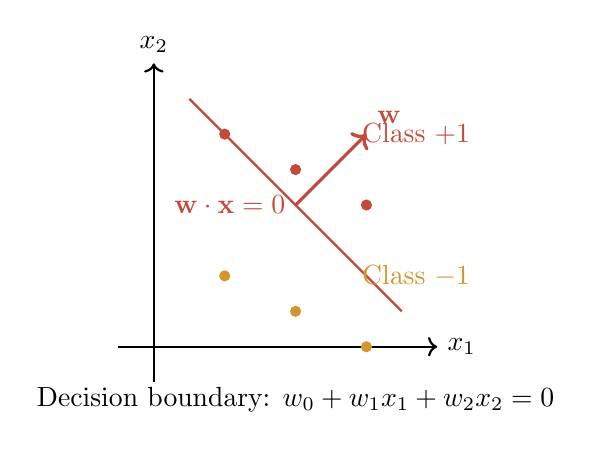
\begin{tikzpicture}[scale=0.9]
    % Axes
    \draw[->, thick] (-0.5,0) -- (4,0) node[right]{$x_1$};
    \draw[->, thick] (0,-0.5) -- (0,4) node[above]{$x_2$};
    % Decision boundary (w0 + w1x1 + w2x2 = 0)
    \draw[wp-primary, thick] (0.5,3.5) -- (3.5,0.5) node[midway, left]{$\mathbf{w}\cdot\mathbf{x}=0$};
    % Weight vector (normal to boundary)
    \draw[->, wp-primary, very thick] (2,2) -- (3,3) node[above right]{$\mathbf{w}$};
    \filldraw[wp-primary] (1,3) circle (2pt);
    \filldraw[wp-primary] (2,2.5) circle (2pt);
    \filldraw[wp-primary] (3,2) circle (2pt);
    \filldraw[wp-accent] (1,1) circle (2pt);
    \filldraw[wp-accent] (2,0.5) circle (2pt);
    \filldraw[wp-accent] (3,0) circle (2pt);
    \node[wp-primary] at (3.7,3) {Class $+1$};
    \node[wp-accent] at (3.7,1) {Class $-1$};
    \node at (2,-0.75) {Decision boundary: $w_0 + w_1x_1 + w_2x_2 = 0$};
\end{tikzpicture}
\end{marginfigure}

This geometric perspective reveals the perceptron's fundamental limitation: it can only learn \textit{linearly separable} functions. The classic XOR problem exemplifies this constraint - no single line can separate $(0,1)$ and $(1,0)$ from $(0,0)$ and $(1,1)$ in $\mathbb{R}^2$. This motivated the development of multilayer perceptrons (MLPs) that can construct nonlinear decision boundaries through composition of multiple hyperplanes.

\paragraph{The XOR Problem}

The "XOR Problem" is a classical problem in Computational Intelligence, proposed initially by Marvin Minsky in his book "Perceptron" (1969). It's the problem of using a Perceptron to predict the output of XOR logic gates given two binary inputs. A XOR function should return true only if the two inputs are not equal.

\begin{figure}[h]
    \centering
    \begin{subfigure}{0.45\textwidth}
        \centering
        \begin{tabular}{c|c|c}
            Input 1 & Input 2 & Output \\
            \hline
            0 & 0 & 0 \\
            \hline
            1 & 0 & 1 \\
            \hline
            0 & 1 & 1 \\
            \hline
            1 & 1 & 0 \\
        \end{tabular}
        \caption{XOR truth table}
        \label{tab:xor}
    \end{subfigure}
    \begin{subfigure}{0.45\textwidth}
        \centering
        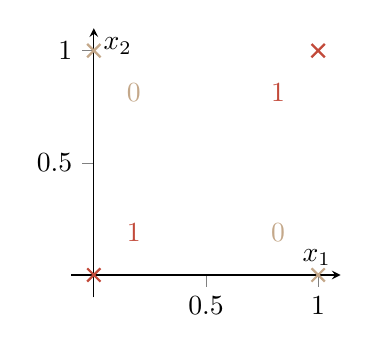
\begin{tikzpicture}
            \tikzstyle{point}=[thick,draw=wp-text,cross out,inner sep=0pt,minimum width=4pt,minimum height=4pt]
            \begin{axis}[
                legend pos=south west,
                axis x line=middle,
                axis y line=middle,
                grid=none,
                width=5cm,
                height=5cm,
                grid style={dashed, wp-muted!30},
                xmin=0, xmax=1, ymin=0, ymax=1,
                xlabel=$x_1$,
                ylabel=$x_2$,
                tick align=outside,
                enlargelimits=true]
              \node[point,label={[label distance=0.3cm,text=wp-muted]135:$0$},wp-muted] at (axis cs:1,0) {};
              \node[point,label={[label distance=0.3cm,text=wp-muted]-45:$0$},wp-muted] at (axis cs:0,1) {};
              \node[point,label={[label distance=0.3cm,text=wp-primary]45:$1$},wp-primary] at (axis cs:0,0) {};
              \node[point,label={[label distance=0.3cm,text=wp-primary]-135:$1$},wp-primary] at (axis cs:1,1) {};
            \end{axis}
        \end{tikzpicture}
        \caption{XOR visualization}
        \label{fig:xor_plot}
    \end{subfigure}
    \caption{XOR operation represented as a truth table (a) and a visualization (b). The plot shows the XOR output for different inputs, where $0$s are marked in \textcolor{wp-muted}{wp-muted} and $1$s are marked in \textcolor{wp-primary}{wp-primary}.}
    \label{fig:xor_combined}
\end{figure}

The structure of a perceptron unit is limited to separating the data points with a single line, and since the XOR inputs are not linearly separable, this cannot be solved. The problem can be solved by adding an extra layer of neurons, called a hidden layer – this architecture is called a Multilayer Perceptron (next section).

\subsection{Activation Functions}

In multilayer networks we need nonlinear, differentiable activation functions. Without nonlinearity, stacking linear layers would still produce only linear functions. Below are the most common activation functions, and Figure~\ref{fig:activations} shows their shapes.

\begin{itemize}
    \item \textbf{Sigmoid}: $\sigma(z) = \frac{1}{1+e^{-z}}$, outputs in $(0,1)$. Smooth but saturates for large $|z|$, causing vanishing gradients.
    \item \textbf{Hyperbolic tangent (tanh)}: $\tanh(z) = \frac{e^{z}-e^{-z}}{e^{z}+e^{-z}}$, outputs in $(-1,1)$. Zero-centered, which helps optimisation, but still saturates.
    \item \textbf{Rectified Linear Unit (ReLU)}: $\text{ReLU}(z) = \max(0,z)$. Non-saturating for $z>0$, computationally efficient, but can cause “dying neurons”.
    \item \textbf{Leaky ReLU}: $\text{LeakyReLU}(z) = \max(\alpha z, z)$ with a small slope $\alpha$ (e.g., $0.01$) for $z<0$, mitigating the dying ReLU problem.
\end{itemize}

\begin{figure}[h]
\centering
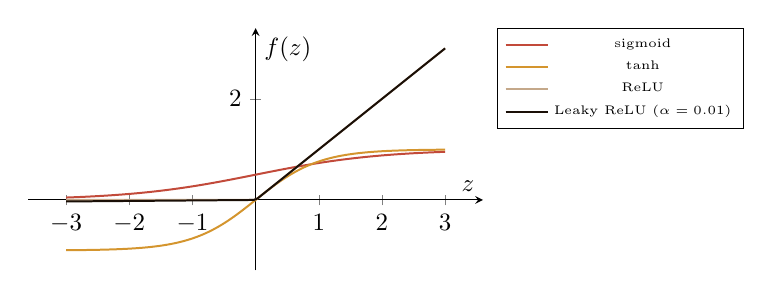
\begin{tikzpicture}[scale=0.9, thick]
    \begin{axis}[
        width=8cm, height=5cm,
        xlabel=$z$,
        ylabel=$f(z)$,
        domain=-3:3,
        samples=100,
        axis lines=middle,
        enlargelimits,
        legend pos=outer north east,
        legend style={font=\tiny}
    ]
        \addplot[wp-primary, thick] {1/(1+exp(-x))};
        \addplot[wp-accent, thick] {tanh(x)};
        \addplot[wp-muted, thick] {max(0,x)};
        \addplot[wp-dark, thick] {max(0.01*x,x)};
        \legend{sigmoid, tanh, ReLU, Leaky ReLU ($\alpha=0.01$)}
    \end{axis}
\end{tikzpicture}
\caption{Common activation functions used in neural networks. Sigmoid and tanh saturate, while ReLU and Leaky ReLU are piecewise linear.}
\label{fig:activations}
\end{figure}

\subsection{Gradient Descent and Stochastic Gradient Descent}

\paragraph{Perceptron Training Rule}
One way to learn an acceptable weight vector is to begin with random weights, then iteratively apply the perceptron to each training example, modifying the perceptron weight whenever it misclassifies an example. This process is repeated, iterating through the training examples as many times as needed until the perceptron classifies all training examples correctly. Weights are modified at each step according to the perceptron training rule, which revises the weight $w_i$ associated with input $x_i$ according to the rule

\begin{equation}
    w_i \leftarrow w_i + \Delta w_i
\end{equation}
where

\begin{equation}
    \Delta w_i = \eta (t - o)x_i
\end{equation}

Here $t$ stands for the target output for the current training example, $o$ is the output generated by the perceptron and $\eta$ is a positive constant called learning rate. The role of the learning rate is to moderate the degree to which weights are changed at each step. It is usually set to some value between 0 and 1, and sometimes made to decay as the number of weight-tuning iterations increases.

\paragraph{Delta Rule}
Although the perceptron rule finds a successful weight vector when the training examples are linearly separable, it can fail to converge if the examples are not linearly separable. A second training rule, called the delta rule, is designed to overcome this problem.
The key idea behind the delta rule is to use gradient descent to search the hypothesis space of possible weight vectors to find the weights that best fit the training examples. This rule sets the basis for the Backpropagation Algorithm.
The delta training rule is best understood by considering the task of training an unthresholded perceptron; that is, a linear unit for which the output $o$ is given by
\begin{equation}
    o(\mathbf{x}) = \mathbf{w} \cdot \mathbf{x}
\end{equation}

Thus, a linear unit corresponds to the first stage of a perceptron, without the threshold.
In order to derive a weight-learning rule for linear units, let us begin by specifying a measure for the training error of a hypothesis, relative to the training examples. Although there are many ways to define the error, one common measure that will turn out to be especially convenient is:
\begin{equation} \label{eq:7}
    E(\mathbf{w}) = \frac{1}{2}\sum_{d\in D} (t_d - o_d)^2
\end{equation}
where $D$ is the set of training examples, $t_d$ is the target output for training example $d$, and $o_d$ is the output of the linear unit for that training example.

\paragraph{Gradient Descent}

To better understand Gradient Descent, it's helpful to visualize the entire hypothesis space of possible weight vectors and their associated $E$ values (Figure \ref{fig:GD}). The Gradient Descent search determines a weight vector that minimizes $E$ by starting with an arbitrary initial weight vector, then repeatedly modifying it in small steps. At each step, the weight vector is altered in the direction that produces the steepest descent along the error surface depicted in Figure \ref{fig:GD}.

\begin{marginfigure}
\centering
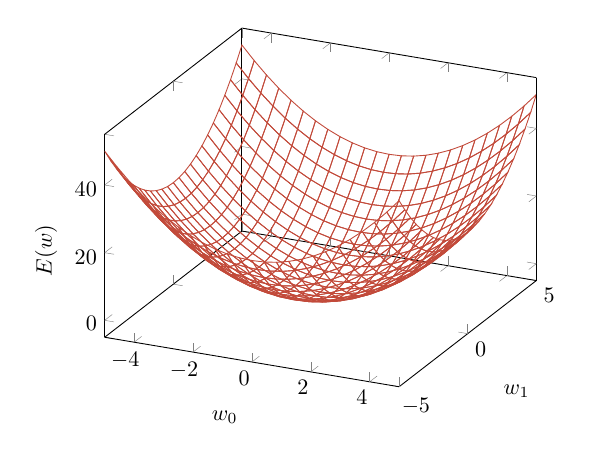
\begin{tikzpicture}[scale=.8, thick]
    \begin{axis}[
        xlabel = {$w_0$},
        ylabel = {$w_1$},
        zlabel = {$E(w)$},
    ]
        \addplot3[
        mesh,
        draw = wp-primary
        ] {x^2 + y^2};
    \end{axis}
\end{tikzpicture}
\caption{Generic representation of a hypothesis space}
\label{fig:GD}
\end{marginfigure}

Based on that, we can calculate the direction of steepest descent along the error surface ($E$) by computing the derivative of $E$ with respect to each component of the vector $\mathbf{w}$. This vector derivative is called the gradient of $E$ with respect to $\mathbf{w}$, written $\nabla E(\mathbf{w})$.
\begin{equation}
    \nabla E(\mathbf{w}) \equiv 
    \left[ \frac{\partial E}{\partial w_0}, \frac{\partial E}{\partial w_1}, ..., \frac{\partial E}{\partial w_n} \right]
\end{equation}
And $\nabla E(\mathbf{w})$ is itself a vector, whose components are the partial derivatives of $E$ with respect to each of the $w_i$. When interpreted as a vector in weight space, the gradient specifies the direction that produces the steepest increase in $E$.
Since the gradient specifies the direction of steepest increase of $E$, the training rule for gradient descent is 
\begin{equation}
    \mathbf{w} \leftarrow \mathbf{w} + \Delta \mathbf{w}
\end{equation}
where
\begin{equation}
    \Delta \mathbf{w} = - \eta \nabla E(\mathbf{w})
\end{equation}
The negative sign is present because we want to move the weight vector in the direction that decreases $E$. This training rule can also be written in its component form

\begin{equation}
    w_i \leftarrow w_i + \Delta w_i
\end{equation}
where
\begin{equation}
    \Delta w_i = -\eta\frac{\partial E}{\partial w_i}
\end{equation}

To efficiently calculate the gradient at each step, we need to obtain the derivatives $\frac{\partial E}{\partial w_i}$ by differentiating $E$ from Equation \ref{eq:7} as:
\begin{equation}
    \begin{split}
        \frac{\partial E}{\partial w_i} &= \frac{\partial}{\partial w_i} \frac{1}{2} \sum_{d \in D} (t_d - o_d)^2 \\
        &= \frac{1}{2} \sum_{d \in D} \frac{\partial}{\partial w_i} (t_d - o_d)^2 \\
        &= \frac{1}{2} \sum_{d \in D} 2 (t_d - o_d) \frac{\partial}{\partial w_i} (t_d - o_d) \\
        &= \sum_{d \in D} (t_d - o_d) \frac{\partial}{\partial w_i} (t_d - \mathbf{w} \cdot \mathbf{x}_d) \\
        &= \sum_{d \in D} (t_d - o_d)(-x_{id})
    \end{split}
\end{equation}

where $x_{id}$ denotes the $i$-th input component for training example $d$. With all that, we now have an equation that gives $\frac{\partial E}{\partial w_i}$ in terms of the linear unit inputs $x_{id}$, outputs $o_d$, and target values $t_d$ associated with the training examples. Thus:

\begin{equation}
    \Delta w_i = \eta \sum_{d \in D} (t_d - o_d)x_{id}
\end{equation}

\paragraph{Stochastic Approximation to Gradient Descent}
Due to its computational complexity, we usually do not use GD directly. The need to use the whole dataset at each iteration makes GD computationally expensive. Therefore, we use a stochastic approximation to gradient descent, mostly called stochastic gradient descent or SGD.
In SGD, instead of using the entire dataset for each iteration, only a single random subset (or a single example) is selected to calculate the gradient and update model parameters. The random selection introduces randomness into the optimization process (“stochastic” stands for being well-described by a random probability distribution). Mathematically it can be described as

\begin{equation}
    w_i := w_i - \eta \nabla Q_i (w)
\end{equation}

The randomness of the technique can also provoke some noise in the gradient, causing some large variations in the gradient.

\subsection{Multilayer Perceptron and Backpropagation}
To address the limitations of a single artificial neuron, which can only represent linear decision boundaries, we explore the concept of a multilayer network. In this approach, multiple fully connected layers are stacked on top of each other, enabling the model to learn and represent more complex, nonlinear decision surfaces.

For learning purposes, we'll address the previous network (perceptron) as a Shallow Neural Network. We call it that way because the only way to increase the number of neurons is adding them \textit{"vertically"} due to the nature of a single layer of neurons. Moreover, in this chapter we'll dive into the evolution of these concepts, from Shallow Neural Networks to Deep Neural Networks and their impacts in the field.

A simple way of making a neural network deeper is to compose shallow neural networks: the output of the first unit becomes the input of the second unit. 

At first sight, we need to decide what type of unit we should use as the basis for constructing multilayer networks. Initially, we might be tempted to choose the linear units discussed before, for which we already derived a gradient descent learning rule. However, multiple layers of cascaded linear units still produce only linear functions. What we need is a unit whose output is a nonlinear function of its inputs, but whose output is also a differentiable function of its inputs – like a sigmoid unit, a tanh unit, or a ReLU unit. Any function can be used as long as it covers all the requirements described above.

\paragraph{Backpropagation Algorithm}
The BP algorithm \textit{learns} the weights for a multilayer network, given a network with a fixed set of units and interconnections. It employs gradient descent to attempt to minimize the squared error between network output values and target values for these outputs.
Because we are considering networks with multiple output units rather than single units as before, we begin by redefining $E$ to sum the errors over all of the network output units:

\begin{equation}
    E(\mathbf{w}) \equiv \frac{1}{2} \sum_{d \in D} \sum_{k \in \text{outputs}} (t_{kd} - o_{kd})^2
\end{equation}

where \textit{outputs} is the set of output units in the network, and $t_{kd}$ and $o_{kd}$ are the target and output values associated with the $k$th output unit and training example $d$.

The learning problem faced by Backpropagation is to search a large hypothesis space defined by all possible weight values for all the units in the network, as illustrated in Figure \ref{fig:GD}. The error in that diagram is replaced by our new definition of $E$, and the other dimensions of the space correspond to all the weights associated with all of the units in the network. As in the case of training a single unit, gradient descent can be used to attempt to find a hypothesis to minimize $E$.

One major difference in the case of multilayer networks is that the error surface can have multiple local minima, in contrast to the single-minimum parabolic error surface we saw in Figure \ref{fig:GD}. This means that gradient descent is guaranteed only to converge toward some local minimum, and not necessarily the global minimum error.

The algorithm proceeds as follows:

\begin{itemize}
    \item Each training example is a pair of the form $\langle \mathbf{x}, \mathbf{t} \rangle$, where $\mathbf{x}$ is the vector of network input values, and $\mathbf{t}$ is the vector of target network output values.
    \item $\eta$ is the learning rate. $n_{in}$ is the number of network inputs, $n_{hidden}$ the number of units in the hidden layer, and $n_{out}$ the number of output units.
    \item The input from unit $i$ into unit $j$ is denoted $x_{ij}$, and the weight from unit $i$ to unit $j$ is denoted $w_{ij}$.
\end{itemize}

The Backpropagation algorithm involves two phases for each training example:

\paragraph{Forward Pass:} 
\begin{enumerate}
    \item Initialize the network by assigning random small values to all weights $w_{ij}$.
    \item Present the input vector $\mathbf{x}$ to the input layer.
    \item Propagate the activations forward through the network using the activation function $o_j = f\big( \sum_i w_{ij} x_{ij} \big)$, where $f$ is a differentiable activation function (e.g., sigmoid or ReLU).
\end{enumerate}

\paragraph{Backward Pass (Error Computation and Weight Update):}
\begin{enumerate}
    \item Compute the error for the output layer: $\delta_k = (t_k - o_k)f'(o_k)$, where $f'(o_k)$ is the derivative of the activation function.
    \item Compute the error for the hidden layer units: $\delta_j = f'(o_j) \sum_k w_{jk} \delta_k$.
    \item Update the weights for each layer using the gradient descent rule:
    \begin{equation}
        w_{ij} \leftarrow w_{ij} + \eta \cdot \delta_j \cdot o_i
    \end{equation}
    where $\eta$ is the learning rate and $o_i$ is the activation of the input to unit $j$.
\end{enumerate}

\paragraph{Repeat:}
Repeat the above steps for each training example until convergence or until a predefined number of iterations is reached. Convergence is achieved when the total error $E(\mathbf{w})$ is sufficiently small or no longer decreases significantly.

This process allows the network to adjust its weights iteratively to minimize the error and improve its performance on the training data. While convergence to a global minimum cannot be guaranteed due to the potential for local minima, this algorithm provides a practical and effective approach for training multilayer neural networks.

\begin{algorithm}[h]
    \caption{Backpropagation Algorithm}
        \textbf{Input:} Training examples $\langle \mathbf{x}, \mathbf{t} \rangle$, where $\mathbf{x}$ is the input vector and $\mathbf{t}$ is the target vector. \\
        \textbf{Output:} Trained weights $w_{ij}$ minimizing the error function. \\
        \textbf{Initialize:} Randomly set all weights $w_{ij}$ to small values. Set the learning rate $\eta > 0$. \\
        
        \textbf{Forward Pass} \\
        1. Present the input vector $\mathbf{x}$ to the network. \\
        2. For each neuron $j$ in hidden and output layers, compute: \\
        \begin{equation*}
            o_j = f\left(\sum_i w_{ij} x_{ij}\right)
        \end{equation*}
        where $f(\cdot)$ is a differentiable activation function (e.g., sigmoid, ReLU). \\
        
        \textbf{Backward Pass} \\
        1. Compute the error signal $\delta_k$ for each output unit $k$: \\
        \begin{equation*}
            \delta_k = (t_k - o_k) f'(o_k)
        \end{equation*}
        2. Compute the error signal $\delta_j$ for each hidden unit $j$: \\
        \begin{equation*}
            \delta_j = f'(o_j) \sum_k w_{jk} \delta_k
        \end{equation*}
        3. Update the weights $w_{ij}$ for each connection: \\
        \begin{equation*}
            w_{ij} \leftarrow w_{ij} + \eta \cdot \delta_j \cdot o_i
        \end{equation*}

        Repeat
        Perform the \textit{Forward Pass} and \textit{Backward Pass} for all training examples. \\
        Until Convergence is achieved (e.g., total error $E(\mathbf{w})$ becomes sufficiently small or stops decreasing).
\end{algorithm}

\newpage

\subsection{Universal Approximation Theorem}
\begin{figure}[h]
\centering
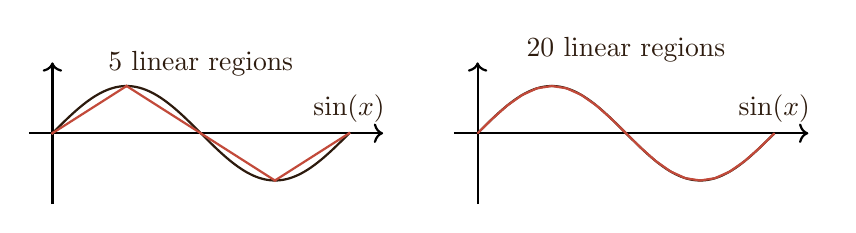
\begin{tikzpicture}[scale=.6, thick]

    % First plot: 5 linear regions
    \begin{scope}[shift={(0, 0)}]
        \draw[->] (-0.5, 0) -- (7, 0) node[right] {};
        \draw[->] (0, -1.5) -- (0, 1.5) node[above] {};

        \draw[wp-text, thick, domain=0:6.28, samples=100, smooth] 
            plot (\x, {sin(\x r)});

        \draw[wp-primary, thick] (0, 0) -- (1.57, 1);
        \draw[wp-primary, thick] (1.57, 1) -- (3.14, 0);
        \draw[wp-primary, thick] (3.14, 0) -- (4.71, -1);
        \draw[wp-primary, thick] (4.71, -1) -- (6.28, 0);

        \node[above] at (6.28, 0) {\textcolor{wp-text}{$\sin(x)$}};
        \node[above] at (3.14, 1) {\textcolor{wp-text}{5 linear regions}};

        \foreach \x/\y in {0/0, 1.57/1, 3.14/0, 4.71/-1, 6.28/0} {
            \fill[wp-primary] (\x, \y) circle (1pt);
        }
    \end{scope}

    % Second plot: 20 linear regions (corrected)
    \begin{scope}[shift={(9, 0)}]
        \draw[->] (-0.5, 0) -- (7, 0) node[right] {};
        \draw[->] (0, -1.5) -- (0, 1.5) node[above] {};

        \draw[wp-text, thick, domain=0:6.28, samples=100, smooth] 
            plot (\x, {sin(\x r)});

        % Draw linear approximation with 20 regions
        \foreach \i in {0,...,19} {
            \pgfmathsetmacro{\xstart}{\i * 6.28 / 20}
            \pgfmathsetmacro{\xend}{(\i + 1) * 6.28 / 20}
            \pgfmathsetmacro{\ystart}{sin(\xstart r)}
            \pgfmathsetmacro{\yend}{sin(\xend r)}
            \draw[wp-primary, thick] (\xstart, \ystart) -- (\xend, \yend);
        }

        \node[above] at (6.28, 0) {\textcolor{wp-text}{$\sin(x)$}};
        \node[above] at (3.14, 1.3) {\textcolor{wp-text}{20 linear regions}};

        \foreach \i in {0,...,20} {
            \pgfmathsetmacro{\x}{\i * 6.28 / 20}
            \pgfmathsetmacro{\y}{sin(\x r)}
            \fill[wp-primary] (\x, \y) circle (0.5pt);
        }
    \end{scope}
\end{tikzpicture}
\caption{Visualization of the Universal Approximation Theorem with 5 and 20 linear regions. More linear regions (more hidden units) allow better approximation of $\sin(x)$.}
\label{fig:UAT}
\end{figure}

George Cybenko published "Approximation by superpositions of a sigmoidal function" proposing a theorem which shows that a finite sum of sigmoidal functions can densely approximate any continuous function in $C(I^n)$ where:
\begin{itemize}
    \item $I^n$: $[0,1]^n$ is the n-dimensional unit cube.
    \item $C(I^n)$: space of continuous functions on $I^n$, with the \textit{supremum} norm $\| \cdot \|$.
\end{itemize}

Cybenko's theorem demonstrates that a neural network with sufficient capacity, even if shallow, can accurately represent any continuous function within a specified range. Usually, Cybenko's theorem is referred to as the case with arbitrary width.

To easily understand the Universal Approximation Theorem (UAT), we can visualize how it works in Figure \ref{fig:UAT}.

\end{document}